\section{Functions and Continuity} 

  Note that from set theory, we can construct functions as a subset of Cartesian product of two spaces $X, Y$. There is nothing new here. 

  \begin{definition}[Continuous Function]
    A function $f$ between 2 topological spaces $(X, \T_{X})$ and $(Y, \T_{Y})$ is \textbf{continuous at $x \in X$} if the preimage of every open neighborhood of $f(x) \in Y$ is an open neighborhood of $x \in X$.
    \begin{equation}
      U_{f(x)} \in \T_{Y} \implies x \in f^{-1}(U_{f(x)}) \in \T_{X}
    \end{equation} 
    $f$ is said to be \textbf{continuous} (at all points) if the preimage of every open set in $Y$ is an open set in $X$.\footnote{Note that continuity of a function $f$ is not only determined by the function itself, but also by the topologies of $X$ and $Y$.}
  \end{definition}

  Note that it is easier for $f$ to be continuous when the $\T_X$ is finer (since there are more open sets in $X$ for the preimage of $V \subset Y$ to map to) or $\T_Y$ is coarser (since there are fewer open sets that we have to check to map to open sets of $X$). 

  \begin{theorem}[Sufficient Properties for Continuity]
    Let $X, Y$, be topological spaces and let $f: X \longrightarrow Y$. Then, the following are equivalent to $f$ being continuous. 
    \begin{enumerate}
      \item The preimage of every basis element $B \in \T_Y$ is open in $X$. 
      \item For every closed set $B$ in $Y$, the set $f^{-1} (B)$ is closed in $X$. 
      \item For every subset $A$ of $X$, $f(\bar{A}) \subset \bar{f(A)}$. 
    \end{enumerate}
  \end{theorem}  
  \begin{proof}
    Listed. 
    \begin{enumerate}
      \item An arbitrary open set $V$ of $Y$ can be written as $V = \cup_{\alpha \in J} b_\alpha$. Then, 
      \begin{equation}
        f^{-1} (V) = f^{-1} \Big( \bigcup_{\alpha \in J} b_\alpha \Big) = \bigcup_{\alpha \in J} f^{-1} (b_\alpha)
      \end{equation}
    \end{enumerate}
  \end{proof}

  Great, so we have a few ways in which we can check continuity of a function. There are a few special cases. 

  \begin{lemma}[Trivially Continuous Functions]
    We have the following for general topological spaces. 
    \begin{enumerate}
      \item The identity function $\id: (X, \T_1) \rightarrow (X, \T_2)$ is continuous if $\T_1 \supset \T_2$. 
      \item A constant function $f: (X, \T) \rightarrow (Y, \T_2)$ is always continuous, regardless of the topologies. 
    \end{enumerate}
  \end{lemma}
  \begin{proof}
    If we take an open set $U \in \T_2$, its preimage is the same set $U$, which is guaranteed to be in $\T_1$ since $\T_1$ is finer than $\T_2$. 
  \end{proof}

  \begin{lemma}[Composition of Continuous Functions]
    If $f: X \rightarrow Y$ and $g: Y \rightarrow Z$ is continuous, then $g \circ f :X \rightarrow Z$ is continuous. 
  \end{lemma}

\subsection{Construction of Continuous Functions} 

  \begin{theorem}[Arithmetic on Real Continuous Functions]
    If $X$ is a topological space, and if $f, g: X \longrightarrow \mathbb{R}$ are continuous, then $f + g$, $f-g$, and $f \cdot g$ are also continuous. $f / g$ is continuous if $g(x) \neq 0$ for all $x \in X$. 
  \end{theorem}

  \begin{theorem}[Analytic Continuity = Topological Continuity] 
    Given metric spaces with their induced metric topologies $(X, \T_X, d_X)$ and $(Y, \T_Y, d_Y)$. The following are equivalent. 
    \begin{enumerate}
      \item $f: X \rightarrow Y$ is continuous at $x$. 
      \item For every $\delta > 0$, there exists an $\epsilon = \epsilon(\delta) > 0$ such that for all $z \in X$, $d_X (x, z) < \epsilon \implies d_Y (f(x), f(x)) < \delta$.\footnote{This is the definition of continuity at a point in analysis.} 
    \end{enumerate}
  \end{theorem}
  \begin{proof}
    ($\rightarrow$) Assume $f$ is continuous according to the $\epsilon - \delta$ definition. Let $U$ be any open set in $Y$ containing the point $y$, and let $x$ be an element in $f^{-1}(U)$ such that $y = f(x)$. We must prove that $f^{-1}(U)$ is also open. Since open sets contain neighborhoods (e.g. open balls) of all of its points, we can claim that, since $U$ is open by assumption, there exists an open ball $B_y$ around $y$ with radius $\epsilon > 0$. This guarantees the existence of a point $z \in U$ such that $\rho(y, z) < \epsilon$ for any $\epsilon > 0$ that we choose. Since $f$ is continuous, for every $\epsilon >0$ that we chose previously, there exists a $\delta >0$ such that $d(x, w) \implies \rho(f(x), f(w)) < \epsilon$. Since $\rho(f(x), f(w)) < \epsilon$, we can conclude that $f(w) \in B_y \subset U$ when $d(x, w) < \delta$. Therefore, $d(x, w) < \delta \implies w \in f^{-1}(U)$. But this is equivalent to saying that if $w \in B_(x, \delta)$, then $w \in f^{-1}(U)$, which means that every single point $x \in f^{-1}(U)$ contains an open ball neighborhood fully contained in $f^{-1}(U)$. So, by definition, $f^{-1}(U)$ is open. 


    ($\leftarrow$) Assume $f^{-1}(U)$ is open when $U$ is an open set in $Y$, i.e. $f$ is continuous under the topological definition. Let us define the open ball 
    \[ B(f(x), \epsilon) \equiv \{ y \in Y \; | \; \rho(f(x), y) < \epsilon\} \in \tau_Y\]
    By our assumption, $f^{-1} \big( B(f(x), \epsilon) \big)$ is an open set in $\tau_X$, and clearly, $x \in f^{-1} \big( B(f(x), \epsilon) \big)$ since $f^{-1}$ maps the point $f(x) \in B(f(x), \epsilon)$ to $x \in f^{-1} \big( B(f(x), \epsilon) \big)$. But since $f^{-1} \big( B(f(x), \epsilon) \big)$ is open, we can construct an open ball around $x$ with radius $\delta$ fully contained within the open set. Moreover, by selecting a point $p \in B(f(x), \delta) \subset f^{-1}\big( B(f(x), \epsilon) \big)$, we can guarantee that $f(p) \in B(f(x), \epsilon)$. This is precisely the $\epsilon - \delta$ definition of continuity. That is, given an $\epsilon > 0$ to be the radius of an open ball $B(f(x), \epsilon)$ in $Y$, we can always choose a $\delta > 0$ to be the radius of the open ball $B(x, \delta)$ in $X$ that is fully contained within the preimage of $B(f(x), \epsilon)$. In mathematical notation, 
    \[ p \in B(x, \delta) \subset f^{-1} \big( B(f(x), \epsilon) \big) \implies f(p) \in f\big( B(x, \delta) \big) \subset B(f(x), \epsilon)\]
    or equivalently in terms of metrics,
    \[ d(x, p) < \delta \implies \rho (f(x), f(p)) < \epsilon\]
  \end{proof} 

\subsection{Sequences}

  \begin{definition}[Sequence]
    A sequence $(x_\alpha)$ of points in topological space $(X, \T)$ is said to \textbf{converge} to the point $x \in X$ if for every neighborhood $U$ of $x$ there exists a $N \in \mathbb{N}$ such that
    \begin{equation}
      x_n \in U \text{ for all } n \geq N
    \end{equation}
  \end{definition}

\subsection{Homeomorphisms}

  \begin{definition}[Homeomorphism]
    A bijective, bicontinuous function $f: X \longrightarrow Y$ between two topological spaces is called a \textbf{homeomorphism} between $X$ and $Y$. If there exists at least one homeomorphism between $X$ and $Y$, then $X$ is said to be \textbf{homeomorphic} to $Y$, denoted $X \cong Y$. 

    \begin{figure}[H]
      \centering 
      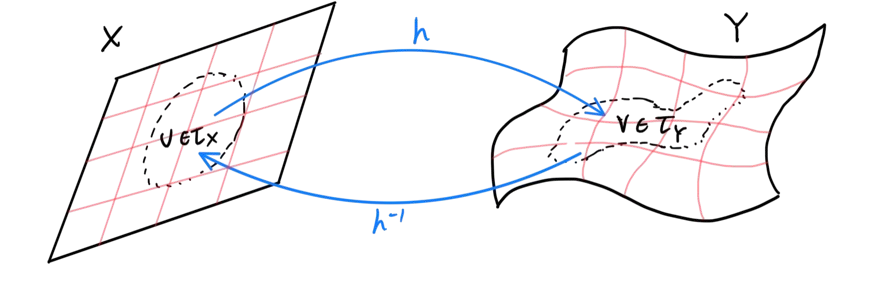
\includegraphics[scale=0.4]{img/Homeomorphism_of_Plane.png}
      \caption{The visual below shows a homeomorphism between the plane $X$ and the surface $Y$.}
      \label{fig:homeomorphism_plane}
    \end{figure}
  \end{definition}

  \begin{theorem}[Sufficient Properties of Homeomorphism]
    Suppose $f: X \rightarrow Y$ is a bijection. TFAE. 
    \begin{enumerate}
      \item $U \subset Y$ is open iff $f^{-1} (U)$ is open. 
      \item $U \subset X$ is open iff $f(U)$ is open. 
      \item $f$ is a homeomorphism. 
    \end{enumerate}
  \end{theorem} 

  Note that we may have functions that are bijective and continuous, but not bicontinuous. In order to construct such examples one of the easiest things we can do is just endow the codomain with the discrete topology, which guarantees continuity. 

  \begin{example}[Bijective and Continuous but not Homeomorphism]
    $\mathbb{Z}$ and $\mathbb{Q}$ are countable sets, so there is a bijection between them. If we give each of them the metric topology, $\mathbb{Z}$ ends up having the discrete topology (take the $0.5$-ball around each integer), whereas for $\mathbb{Q}$, we will see later that by the density of the rationals there are an infinite number of rationals in $(q - r, q + r)$ for $q \in \mathbb{Q}$. Note that this bijection $f: \mathbb{Z} \rightarrow \mathbb{Q}$ is continuous (since $\mathbb{Z}$ has discrete topology) but not bicontinuous. 
  \end{example}


  \begin{example}[Comparability and Homeomorphic Spaces]
    Consider the set $X = \{a, b\}$ with the two topologies $\T_3 = \{\emptyset, \{a\}, X\}$ and $\T_4 = \{\emptyset, \{b\}, X\}$. They are not comparable but they seem ``similar'' in a way in that if we swap all the $a$'s and $b$'s in $\T_3$, then we get $\T_4$. We can make this rigorous by defining $f: (X, \T_3) \rightarrow (X, \T_4)$ with $f(a) = b, f(b) = a$, and showing that it is a homeomorphism. 
  \end{example}

  In fact, a homeomorphism $f$ is an equivalence relation between two topological spaces. This partitions the set of all topological spaces into \textbf{homeomorphism classes}. Analogous to how isomorphisms preserve algebraic structures, homeomorphisms preserve topological structure between topological spaces. 

  \begin{example}[Homeomorphism Classes of 2D Manifolds]
    There is an infinite family of 2-dimensional manifolds, call them $M$ and $N$, and each set in each family is not homeomorphic to another.  
    \begin{enumerate}
      \item $M_0 = S^2$ (sphere). $M_1 = T^2$ (torus). $M_2$ is a donut with two holes. $M_3$ has three holes, and so on. 
      \item $N_1$ is the Mobius strip. $N_2$ is the Klein bottle. 
    \end{enumerate}
  \end{example}

  Additionally, not only does a homeomorphism give a bijective correspondence between points in $X$ and $Y$, but it also determines a bijection between \textbf{the set of all open sets in $X$ and $Y$} (that is, a bijection between their topologies)! This bijection then allows two spaces that are homeormophic to have the same topological properties. 

  \begin{theorem}[Preservation of Topological Properties]
    A homeomorphism $f$ between two topological spaces $(X, \tau_{x})$ and $(Y, \tau_{Y})$ preserves all topological properties (e.g. separability, countability, compactness, (path) connectedness) of $X$ onto $Y$ and $Y$ onto $X$. 
  \end{theorem}

  \begin{definition}[Embedding]
    Suppose that $f: X \longrightarrow Y$ an injective continuous map with $X, Y$ topological spaces. Let $Z \equiv \im{f}$. Then, the function
    \begin{equation}
      f^\prime: X \longrightarrow Z \subset Y
    \end{equation}
    obtained by restricting the codomain of $f$ is bijective. If $f^\prime$ happens to be a homeomorphism of $X$ with $Z$, then we say that the map
    \begin{equation}
      f: X \longrightarrow Y
    \end{equation}
    is a \textbf{topological embedding}, or more simply an \textbf{embedding}, of $X$ in $Y$. 
  \end{definition} 

  A homeomorphism can be useful, but we can work a lot more flexibly with it by knowing that the restriction of a homeomorphism is a homeomorphism. 

  \begin{theorem}[Restriction of Homeomorphism is Homeomorphism]
    If $f: X \rightarrow Y$ is a homeomorphism, then for any $x \in X$, the restriction 
    \begin{equation}
      f|_{X \setminus \{x\}} : X \setminus \{x\} \rightarrow Y \setminus \{f(x)\}
    \end{equation}
    is also a homeomorphism. 
  \end{theorem}

\subsection{Hausdorff Axiom (To be Moved)} 

  \begin{lemma} 
    For any metric space, the metric topology is Hausdorff. 
  \end{lemma}

  \begin{lemma} 
    $X$ Hausdorff implies any sequences converges to at most one point. 
  \end{lemma}

  \begin{lemma} 
    $X$ Hausdorff implies any finite subset is closed. 
  \end{lemma}

  \begin{example}
    $X$ is an infinite set, then finite complement topology is not Hausdorff. 
  \end{example} 

  \begin{definition}
    One point sets are closed is the $T_1$ axiom. Equivalently, for any pair $x_1 \neq x_2$, there is an open set $U$ s.t. $x_1 \in U$ and $x_2 \not\in U$. 
  \end{definition}

  \begin{example}[Line with Two Origins]
    $X = \mathbb{R} \setminus \{0\} \cup \{0_1, 0_2\}$ with basis given by intervals $(a, b)$ for $b < 0$ or $a > 0$, and $(a, 0) \cup \{0_i\} \cup (0, b)$ for $a < 0 < b$. 
  \end{example}

\subsection{Exercises}

  \begin{exercise}[Munkres 18.1]
    Prove that for functions $f : \mathbb{R} \to \mathbb{R}$, the $\epsilon$-$\delta$ definition of continuity implies the open set definition.
  \end{exercise}

  \begin{exercise}[Munkres 18.2]
    Suppose that $f : X \to Y$ is continuous. If $x$ is a limit point of the subset $A$ of $X$, is it necessarily true that $f(x)$ is a limit point of $f(A)$?
  \end{exercise}
  \begin{solution}
    No. Consider $X = Y = \mathbb{R}$ with the Euclidean topology and let $f(x) = 0$. Consider $A = (-1, 1) \implies f(A) = \{0\}$. $1$ is a limit point of $A$ but $f(1) = 0$ is not a limit point of $\{0\}$ since it's an isolated point, i.e. for any punctured open neighborhood $U_0^\circ = U_0 \setminus \{0\}$, 
    \begin{equation}
      U_0^\circ \cap f(A) = (U_0 \setminus \{0\}) \cap \{0\} = \emptyset
    \end{equation}
  \end{solution}

  \begin{exercise}[Munkres 18.3]
    Let $X$ and $X'$ denote a single set in the two topologies $\mathcal{T}$ and $\mathcal{T}'$, respectively. Let $i : X' \to X$ be the identity function.
    \begin{enumerate}
      \item Show that $i$ is continuous $\Leftrightarrow \mathcal{T}'$ is finer than $\mathcal{T}$.
      \item Show that $i$ is a homeomorphism $\Leftrightarrow \mathcal{T}' = \mathcal{T}$.
    \end{enumerate}
  \end{exercise}

  \begin{exercise}[Munkres 18.4]
    Given $x_0 \in X$ and $y_0 \in Y$, show that the maps $f : X \to X \times Y$ and $g : Y \to X \times Y$ defined by
    \begin{align*}
      f(x) = x \times y_0 \quad \text{and} \quad g(y) = x_0 \times y
    \end{align*}
    are imbeddings.
  \end{exercise}

  \begin{exercise}[Munkres 18.5]
    Show that the subspace $(a, b)$ of $\mathbb{R}$ is homeomorphic with $(0, 1)$ and the subspace $[a, b]$ of $\mathbb{R}$ is homeomorphic with $[0, 1]$.
  \end{exercise}

  \begin{exercise}[Munkres 18.6]
    Find a function $f : \mathbb{R} \to \mathbb{R}$ that is continuous at precisely one point.
  \end{exercise}

  \begin{exercise}[Munkres 18.7]
    \begin{enumerate}
      \item Suppose that $f : \mathbb{R} \to \mathbb{R}$ is ``continuous from the right,'' that is,
      \begin{align*}
        \lim_{x \to a^+} f(x) = f(a),
      \end{align*}
      for each $a \in \mathbb{R}$. Show that $f$ is continuous when considered as a function from $\mathbb{R}_\ell$ to $\mathbb{R}$.
      \item Can you conjecture what functions $f : \mathbb{R} \to \mathbb{R}$ are continuous when considered as maps from $\mathbb{R}$ to $\mathbb{R}_\ell$? As maps from $\mathbb{R}_\ell$ to $\mathbb{R}_\ell$? We shall return to this question in Chapter 3.
    \end{enumerate}
  \end{exercise}
  \begin{solution}
    This definition of continuity at a point in analysis means that for all $\epsilon > 0$ there exists a $\delta > 0$ s.t. $x \in [a, a + \delta) \implies |f(x) - f(a)| < \epsilon$. Assuming this definition holds, let $U_{f(a)} \in \T$ be an open neighborhood of $f(a)$ (w.r.t. Euclidean topology). We wish to show that the preimage is open in $\T_\ell$. 

    By definition of open sets in $\mathbb{R}$, there exists an open ball $(f(a) - \epsilon, f(a) + \epsilon) \subset U_{f(a)}$, and from our analytical definition of continuity there exists a $\delta > 0$ s.t. $f([a, a + \delta)) \subset (f(a) - \epsilon, f(a) + \epsilon)$. Therefore taking the preimage we have 
    \begin{equation}
      [a, a+\delta) \subset f^{-1} \big( (f(a) - \epsilon, f(a) + \epsilon ) \big) \subset f^{-1} \big( U_{f(a)} \big)
    \end{equation}
    Since we can construct an open ball (in $\T_\ell$) $[a, a + \delta) \subset f^{-1} (U_{f(a)})$, by definition $f^{-1} (U_{f(a)})$ is open in $\mathbb{R}_\ell$, making $f$ continuous at $a$. Since this holds for all $a$, $f$ is continuous.\footnote{We could have started off with an arbitrary open set $U$ and chosen an arbitrary $a \in f^{-1} (U)$ to get the same result.} 
  \end{solution}

  \begin{exercise}[Munkres 18.8]
    Let $Y$ be an ordered set in the order topology. Let $f, g : X \to Y$ be continuous.
    \begin{enumerate}
      \item Show that the set $\{x \mid f(x) \leq g(x)\}$ is closed in $X$.
      \item Let $h : X \to Y$ be the function
      \begin{align*}
        h(x) = \min\{f(x), g(x)\}.
      \end{align*}
      Show that $h$ is continuous. [Hint: Use the pasting lemma.]
    \end{enumerate}
  \end{exercise}

  \begin{exercise}[Munkres 18.9]
    Let $\{A_\alpha\}$ be a collection of subsets of $X$; let $X = \bigcup_\alpha A_\alpha$. Let $f : X \to Y$; suppose that $f|A_\alpha$ is continuous for each $\alpha$.
    \begin{enumerate}
      \item Show that if the collection $\{A_\alpha\}$ is finite and each set $A_\alpha$ is closed, then $f$ is continuous.
      \item Find an example where the collection $\{A_\alpha\}$ is countable and each $A_\alpha$ is closed, but $f$ is not continuous.
      \item An indexed family of sets $\{A_\alpha\}$ is said to be \textit{locally finite} if each point $x$ of $X$ has a neighborhood that intersects $A_\alpha$ for only finitely many values of $\alpha$. Show that if the family $\{A_\alpha\}$ is locally finite and each $A_\alpha$ is closed, then $f$ is continuous.
    \end{enumerate}
  \end{exercise}

  \begin{exercise}[Munkres 18.10]
    Let $f : A \to B$ and $g : C \to D$ be continuous functions. Let us define a map $f \times g : A \times C \to B \times D$ by the equation
    \begin{equation}
      (f \times g)(a \times c) = f(a) \times g(c).
    \end{equation}
    Show that $f \times g$ is continuous.
  \end{exercise}
  \begin{solution}
    Let $V$ be an open set in $B \times D$. Then $V$ can be expressed as the union of basis elements in the product topology, with the form 
    \begin{equation}
      V = \bigcup U_B \times U_D
    \end{equation}
    where $U_B \in \mathscr{T}_B$ and $U_D \in \mathscr{T}_D$. Now take the preimage. 
    \begin{equation}
      (f \times g)^{-1} (V) = \bigcup (f \times g)^{-1} (U_B \times U_D) = \bigcup f^{-1}(U_B) \times g^{-1} (U_D)
    \end{equation}
    Since $f, g$ are continuous, $f^{-1} (U_B) \in \mathscr{T}_A$ and $g^{-1} (U_D) \in \mathscr{T}_C$. Therefore, $f^{-1} (U_B) \times g^{-1} (U_D)$ is a basis element of the product topology $\mathscr{T}_{A \times C}$, and its arbitrary union is indeed an open set in $A \times C$. Therefore $f \times g$ is continuous.  
  \end{solution}

  \begin{exercise}[Munkres 18.11]
    Let $F : X \times Y \to Z$. We say that $F$ is \emph{continuous in each variable separately} if for each $y_0$ in $Y$, the map $h : X \to Z$ defined by $h(x) = F(x \times y_0)$ is continuous, and for each $x_0$ in $X$, the map $k : Y \to Z$ defined by $k(y) = F(x_0 \times y)$ is continuous. Show that if $F$ is continuous, then $F$ is continuous in each variable separately.
  \end{exercise}
  \begin{solution}
    Let us define $\iota_{y_0}: X \rightarrow X \times Y$ as the canonical injection $\iota_{y_0}(x) = (x, y_0)$. We first show that this is continuous. First choose an open set $V \in \mathscr{T}_{X \times Y}$, which is of the form 
    \begin{equation}
      V = \bigcup U_X \times U_Y
    \end{equation}
    for open sets $U_X \in \mathscr{T}_X, U_Y \in \mathscr{T}_Y$. Taking the preimage 
    \begin{equation}
      \iota_{y_0}^{-1} (V) = \bigcup \iota_{y_0}^{-1} (U_X \times U_Y)
    \end{equation}
    For each term in the union, note that if $y_0 \not\in U_Y$, then the preimage is $\emptyset$, which is open. If $y_0 \in U_Y$, then the preimage is $U_X$ which is open. Therefore the union of such open sets is open. With this, note that 
    \begin{equation}
      h = F \circ \iota_{y_0}
    \end{equation}
    which is a composition of continuous maps and therefore is continuous. The proof for $k$ is identical. 
  \end{solution}

  \begin{exercise}[Munkres 18.12]
    Let $F : \mathbb{R} \times \mathbb{R} \to \mathbb{R}$ be defined by the equation
    \begin{equation}
      F(x \times y) = \begin{cases}
        xy/(x^2 + y^2) & \text{if } x \times y \neq 0 \times 0, \\
        0              & \text{if } x \times y = 0 \times 0.
      \end{cases}
    \end{equation}
    \begin{enumerate}
      \item Show that $F$ is continuous in each variable separately.
      \item Compute the function $g : \mathbb{R} \to \mathbb{R}$ defined by $g(x) = F(x \times x)$.
      \item Show that $F$ is not continuous.
    \end{enumerate}
  \end{exercise}
  \begin{solution}
    \begin{enumerate}
      \item Fix $y = y_0$. Then if $y_0 = 0$, $h(x) = 0$ which is continuous. If $y_0 \neq 0$, then 
      \begin{equation}
        h(x) = F(x \times y_0) = \frac{y_0 x}{x^2 + y_0^2}
      \end{equation}
      which is the quotient of two polynomials, which are continuous, and the denominator never vanishes since $x^2 + y_0^2 \geq y_0^2 > 0$. Similarly, if we fix $x = x_0$, $k(y) = 0$ if $x_0 = 0$ and 
      \begin{equation}
        k(y) = F(x_0 \times y) = \frac{x_0 y}{y^2 + x_0^2}
      \end{equation}
      which is the quotient of two polynomials where the denominator never vanishes. 

      \item We have 
      \begin{equation}
        g(x) = \begin{cases} 
          F(0) = 0 & \text{ if } x = 0 \\
          F(x \times x) = \frac{x^2}{2 x^2} = \frac{1}{2} & \text{ if } x \neq 0
        \end{cases}
      \end{equation}

      \item We see that $g$ above is not continuous since the preimage of the open set $(-0.25, 0.25)$ is $\{0\}$ which is not open. We can write $g = F \circ \iota$, where $\iota(x) = (x, x)$. We claim that $\iota$ is continuous. Take any basis element $U \times V \in \mathscr{T}_{X \times X}$ where $U, V$ are open in $X$. The preimage consists of all points $x$ that are both in $U$ and $V$, i.e. $\iota^{-1} (U \times V) = U \cap V$, which is open.  Therefore $\iota$ is continuous. If $F$ was continuous, then $F \circ \iota$ would be continuous, but $g$ is not continuous, so $F$ must not be continuous. 
    \end{enumerate}
  \end{solution}

  \begin{exercise}[Munkres 18.13]
    Let $A \subset X$; let $f : A \to Y$ be continuous; let $Y$ be Hausdorff. Show that if $f$ may be extended to a continuous function $g : \bar{A} \to Y$, then $g$ is uniquely determined by $f$.
  \end{exercise}
  \begin{solution}
    Let us consider two such extensions $g, h$. If $A = \overline{A}$, then $g = f = h$ and this is unique. If $A \subsetneq \overline{A}$ then there exists $x \in A^\prime \setminus A$. Since $Y$ is Hausdorff, there exists disjoint open neighborhoods $U \ni g(x), V \ni h(x)$. It is the case that $x \in g^{-1}(U) \cap h^{-1} (V)$ open (since $f, h$ are continuous and so their preimages are open). Since $x$ is a limit point of $A$, there exists a $y \in g^{-1} (U) \cap h^{-1} (V) \cap A$ not equal to $x$. Mapping through through $h, g$ again gives $g(y) \in U$, $h(y) \in V$. But since $y \in A$, the two must agree with $f$, and so $f(y) = g(y) = h(y)$, which contradicts that $Y$ is Hausdorff. 
  \end{solution}

  \begin{exercise}[Math 411 Spring 2025, PS4]
    Suppose $X$ and $Y$ are topological spaces, where $Y$ is Hausdorff, and let $f$ and $g$ be continuous functions from $X$ to $Y$. Prove that the set $S = \{x \in X \mid f(x) = g(x)\}$ is closed.
  \end{exercise}
  \begin{solution}
    We equivalently wish to show that $X \setminus S$ is open. For any $x \in (X \setminus S)$, we have $f(x) \neq g(x) \in Y$. Since $Y$ is Hausdorff, there exists open $U_{f(x)} \ni f(x)$ and open $U_{g(x)} \ni g(x)$ s.t. $U_{f(x)} \cap U_{g(x)} = \emptyset$. Therefore, we can take their preimage $f^{-1} (U_{f(x)}), g^{-1} (U_{g(x)})$ which is open in $X$ by continuity of $f, g$. Furthermore we can take their intersection to get another open neighborhood of $x$. 
    \begin{equation}
     V_x = f^{-1} (U_{f(x)}) \cap g^{-1} (U_{g(x)}) 
    \end{equation}
    We claim that $V_x \cap S = \emptyset$. Assuming not, we have some $s \in V_x \cap S$. Since $s \in V_x$, $f(s) \in U_{f(x)}$ and $g(s) \in U_{g(x)}$, but since $s \in S$, $f(x) = g(x)$ and these map to the same point, contradicting the fact that $U_{f(x)}$ and $U_{g(x)}$ are disjoint. Therefore, our claim holds true, which implies that $V_x \subset X \setminus S$. Therefore, we have proved that all points $x \in (X \setminus S)$ is an interior point, and thus $X \setminus S$ is open.\footnote{This can be shown by letting $X \setminus S$ be the union of all $V_x$ for $x \in (X \setminus S)$ which is open.}
  \end{solution}

  \begin{exercise}[Math 411 Spring 2025, PS5]
    Let $X$ be a topological space, and let $f,g: X \to \mathbb{R}$ be continuous maps.
    \begin{enumerate}
      \item Show that the set $\{x \in X \mid f(x) \leq g(x)\}$ is closed in $X$.
      
      \item Show that the function $h: X \to \mathbb{R}$ given by $h(x) = \max\{f(x),g(x)\}$ is continuous.
    \end{enumerate}
    
    \noindent\textbf{Note:} If you prefer, instead of $\mathbb{R}$ you can use an arbitrary ordered set $Y$ with the order topology in place of $Y$, as in \S18 \#8. (We did not cover the order topology in class; see \S14 if you're curious.)
  \end{exercise}
  \begin{solution}
    For any $y \in \mathbb{R}$. The sets $\{x \in X \mid f(x) > y\}$ and $\{x \in X \mid y > g(x)\}$ are open since they are the preimages of $(y, +\infty)$ and $(-\infty, y)$ respectively. Therefore their intersection is open, i.e. 
    \begin{equation}
      U_y = \{x \in X \mid f(x) > y > g(x)\}
    \end{equation} 
    Therefore their union is also open. 
    \begin{equation}
      U = \bigcup_{y \in \mathbb{R}} U_y = \{x \in X \mid f(x) > g(x)\}
    \end{equation}
    where we can always identify a $y = (f(x) + g(x))/2$. Therefore the complement where $f(x) \leq g(x)$ is closed. 
    
    As for the second part, we will denote $U_f = \{x \in X \mid f(x) \leq g(x)\}$ and $U_g = \{x \in X \mid g(x) \geq f(x) \}$. They are both closed, where $U_g$ can be proved closed by the same symmetric argument. Let us take any closed set $S \subset X$. Since $X = U_f \cup U_g$, we can denote 
    \begin{equation}
      S = S \cap X = S \cap (U_f \cup U_g) = (S \cap U_f) \cup (S \cap U_g) = V_f \cup V_g
    \end{equation}
    where $V_f, V_g$ are closed since we proved before that $U_f, U_g$ are closed. The preimage is 
    \begin{align}
      h^{-1} (S) & = h^{-1} (V_f) \cup h^{-1} (V_g) \\
                 & = g^{-1} (V_f) \cup f^{-1} (V_g)
    \end{align}
    which is the union of open sets and therefore open. 
  \end{solution}


